%% ============================================================
% f2012_sichuan_arts_q05_square.tex
%% 2012 四川卷（文科）第 5 题 正方形 ABCD，延长 BA 至 E 使 AE=1
%% 来源 PDF：普通高考/2012/2012四川文.pdf 第 1 页（印面 773）第 1 栏
%% 坐标取自原页矢量层（bp），原点为图区左上角 (175.0,635.0)，y 向下。
%% ============================================================
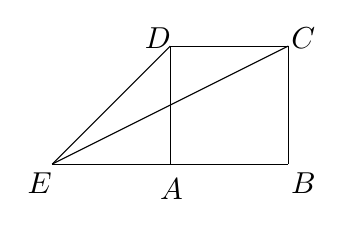
\begin{tikzpicture}[x=1bp,y=-1bp,
  every node/.style={inner sep=0,font=\fontsize{10.5pt}{12.6pt}\selectfont},
  line cap=butt, line join=miter]
  \draw[line width=0.398bp] (5.828,49.738) -- (90.836,49.738);
  \draw[line width=0.398bp] (90.836,7.234) -- (48.332,7.234);
  \draw[line width=0.398bp] (5.828,49.738) -- (90.836,7.234);
  \draw[line width=0.398bp] (90.836,49.738) -- (90.836,7.234);
  \draw[line width=0.398bp] (5.828,49.738) -- (48.332,7.234);
  \draw[line width=0.398bp] (48.332,49.738) -- (48.332,7.234);
  \node[anchor=base west] at (38.99,8.07) {$D$};
  \node[anchor=base west] at (91.74,8.07) {$C$};
  \node[anchor=base west] at (-3.21,60.45) {$E$};
  \node[anchor=base west] at (44.48,62.49) {$A$};
  \node[anchor=base west] at (91.62,60.45) {$B$};
\end{tikzpicture}
